%%%%%%%%%%%%%%%%%%%%%%%%%%%%%%%%%%%%%%%%%%%%%%%%%%%%%%%%%%%%%%%%%%%%%%%%%%

% abnTeX2: Modelo de Trabalho Acadêmico em conformidade com 
% as normas da ABNT

%%%%%%%%%%%%%%%%%%%%%%%%%%%%%%%%%%%%%%%%%%%%%%%%%%%%%%%%%%%%%%%%%%%%%%%%%%

\documentclass[english, 
               brazil, 
               bsc] %Opções bsc (TCC) e msc (Mestrado)
               {dcomp-abntex2}


%%%%%%%%%%%%%%%%%%%%%%%%%%%%%%%%%%%%%%%%%%%%%%%%%%%%%%%%%%%%%%%%%%%%%%%%%%
% Área para adição de pacotes extras
%%%%%%%%%%%%%%%%%%%%%%%%%%%%%%%%%%%%%%%%%%%%%%%%%%%%%%%%%%%%%%%%%%%%%%%%%%

\usepackage{lipsum} %Retirar para a versão final do documento

%Utilize aqui seu pacote preferido para algoritmos
\usepackage[linesnumbered]{algorithm2e}

%%%%%%%%%%%%%%%%%%%%%%%%%%%%%%%%%%%%%%%%%%%%%%%%%%%%%%%%%%%%%%%%%%%%%%%%%%

%Compila o indice
\makeindex

\begin{document}

% Seleciona o idioma do documento (conforme pacotes do babel)
\selectlanguage{brazil}

% Retira espaço extra obsoleto entre as frases.
\frenchspacing 

%%%%%%%%%%%%%%%%%%%%%%%%%%%%%%%%%%%%%%%%%%%%%%%%%%%%%%%%%%%%%%%%%%%%%%%%%%
% ELEMENTOS PRÉ-TEXTUAIS
%%%%%%%%%%%%%%%%%%%%%%%%%%%%%%%%%%%%%%%%%%%%%%%%%%%%%%%%%%%%%%%%%%%%%%%%%%

\pretextual

% \titulo{Desenvolvendo aplicações com arquitetura de microserviços usando o framework DevOps} 
\titulo{Características, padrões e soluções de desenvolvimento de aplicações com arquitetura de microserviços}
\autor{João Paulo Feitosa Secundo}
\orientador{Rafael Oliveira Vasconcelos}
\coorientador{}
\curso{Ciência da Computação}

\inserirInformacoesPDF

\imprimircapa
\imprimirfolhaderosto*

% \include{Pre_Textual/Dedicatoria}
% \begin{agradecimentos}

Teste agradecimentos

\end{agradecimentos}
% ---
% \include{Pre_Textual/Epigrafe}
% % resumo em português
\setlength{\absparsep}{18pt} % ajusta o espaçamento dos parágrafos do resumo
\begin{resumo}

O presente trabalho analisa o desenvolvimento de aplicações com arquitetura de microsserviços, expondo as características desta abordagem arquitetural e reunindo e discutindo práticas usadas no desenvolvimento de aplicações que a usa, por meio de pesquisa e revisão bibliográfica. Também serão discutidas e usadas algumas ferramentas para o desenvolvimento de uma aplicação de exemplo. O resultado é um conjunto de características comuns, práticas bem consolidadas e ferramentas úteis no desenvolvimento de tais aplicações. Ademais, foi identificado que certas práticas têm circunstâncias subjetivas e devem ser ponderadas antes de aplicadas, pois nem sempre são consideradas favoráveis, por vezes sendo julgadas positivas por alguns autores e negativas por outros.

% Ademais, foi identificado certo nível de discordância entre autores respeitados nesta área sobre a prática de começar a aplicação por uma abordagem arquitetural mais simples, tal como a monolítica, antes de adotar os microsserviços, questão em que há mais espaço para discussões e estudos de caso. 

% Segundo a \citeonline[3.1-3.2]{NBR6028:2003}, o resumo deve ressaltar o objetivo, o método, os resultados e as conclusões do documento. A ordem e a extensão destes itens dependem do tipo de resumo (informativo ou indicativo) e do tratamento que cada item recebe no documento original. O resumo deve ser precedido da referência do documento, com exceção do resumo inserido no próprio documento. (\ldots) As palavras-chave devem figurar logo abaixo do resumo, antecedidas da expressão Palavras-chave:, separadas entre si por ponto e finalizadas também por ponto.

 \textbf{Palavras-chave}: arquitetura de \emph{software}. microsserviços. desenvolvimento. práticas. ferramentas.
\end{resumo}
% % resumo em inglês
\setlength{\absparsep}{18pt} % ajusta o espaçamento dos parágrafos do resumo
\begin{resumo}[Abstract]
 \begin{otherlanguage*}{english}
   This paper analyzes the development of applications with microservice architecture, exposing the characteristics of this architectural approach and gathering and discussing practices used in the development of applications that use it, through literature research and review. Some tools will also be discussed and used for the development of an example application. The result is a set of common characteristics, well established practices and useful tools in the development of such applications. Furthermore, it has been identified that certain practices have subjetive circumstances and must be pondered before applied, for they are not always considered favorable, sometimes being judged positive by some authors and negative by others.
   
  %  it has been identified a certain level of disagreement between respected authors in this area about the practice of starting with a simpler architectural approach, such as the monolithic one, before utilizing microservices, issue in which there is more space for discussions and case studies.

   \vspace{\onelineskip}
 
   \noindent 
   \textbf{Keywords}: software architecture. microservices development. practices. tools.
 \end{otherlanguage*}
\end{resumo}


% \mostrarlistadeILUSTRACOES
% \mostrarlistadeQUADROS
% \mostrarlistadeTABELAS
% \mostrarlistadeCODIGOS
% \mostrarlistadeALGORITMOS
 
% Lista de abreviaturas e siglas

\begin{siglas}
	\item[API]{Application Programing Interface - Interface para programação de aplicação}
	\item[HTTP]{HyperText Transfer Protocol - Protocolo de transferência de hipertexto}
	\item[AMS]{Arquitetura de microsserviços}
	\item[DoS]{Denial of Service - Negação de serviço}
	\item[RFC]{Request For Comments - Pedido de comentários}
	\item[JSON]{JavaScript Object Notation - Notação de objeto javaScript}
	\item[DDD]{Domain-driven Design - Projeto orientado a domínio}
	\item[SSL]{Secure Socket Layer - Camada de soquete seguro}
\end{siglas}
% \include{Pre_Textual/Simbolos}
    
\mostrarSUMARIO

%%%%%%%%%%%%%%%%%%%%%%%%%%%%%%%%%%%%%%%%%%%%%%%%%%%%%%%%%%%%%%%%%%%%%%%%%%
% ELEMENTOS TEXTUAIS
%%%%%%%%%%%%%%%%%%%%%%%%%%%%%%%%%%%%%%%%%%%%%%%%%%%%%%%%%%%%%%%%%%%%%%%%%%

\textual
\chapter{Introdução}\label{chapter-introducao}

O crescimento da Internet e a onipresença da computação móvel tem mudado o jeito como \emph{software} é desenvolvido nos últimos tempos. Todos que têm contato com a área do desenvolvimento de \emph{software} provavelmente conhecem o termo \emph{SaaS (Software as a Service)}, ou \emph{software} como um serviço. Entretanto, essa expressão significa mais do que apenas um modelo de negócio. A tendência que tem-se observado na indústria do \emph{software} é a de oferecer \emph{software} não mais como um pacote completo e fechado, mas sim como um pacote flexível e em constante melhoria, o que implica na mudança do foco dos desenvolvedores para a criação de aplicações modulares, e que permitam que mudanças sejam desenvolvidas e implantadas rápida, fácil e independentemente \cite{CAOPLE, oracle_microservices}.

Essa mudança de foco implicou no surgimento de novas abordagens de arquitetura e organização de \emph{software}, e uma dessas tem ganho grande popularidade na indústria do \emph{software} por facilitar a criação de aplicações que são multilíngues, facilmente mantidas e implantadas, escaláveis, e altamente disponíveis. Inspirada na arquitetura orientada a serviços, ela se chama arquitetura de microsserviços, e é considerada por muitos profissionais da engenharia de \emph{software} como a melhor maneira de arquitetar uma aplicação de \emph{software} como um serviço atualmente. Entretanto, como tudo na computação, há um \emph{trade-off} (uma troca), pois assim como há benefícios, também há desvantagens e desafios no emprego de uma arquitetura de microsserviços, os quais também são discutidos neste trabalho \cite{middleware-microservices,design-monitoring-testing-waseem}.


% Many development teams have found the microservices architectural style to be a superior approach to a monolithic architecture. But other teams have found them to be a productivity-sapping burden. Like any architectural style, microservices bring costs and benefits. To make a sensible choice you have to understand these and apply them to your specific context. microservice tradeoffs - https://martinfowler.com/articles/microservice-trade-offs.html#summary

%Se você quiser projetar um aplicativo que seja multilíngue, facilmente escalável, fácil de manter e implantar, altamente disponível e que minimize falhas, use a arquitetura microservices para projetar e implantar um aplicativo em nuvem. Em uma arquitetura de microservices, cada microservice possui uma tarefa simples e se comunica com os clientes ou com outros microservices usando mecanismos de comunicação leves, como solicitações de API REST. \cite{oracle_microservices}

% O público alvo e os usuários desses softwares podem chegar a números imensos.

% In recent years, the rise of the internet and the ubiquity of mobile computing have made it necessary for application developers to design their applications focusing on a lightweight, self-contained component. Developers need to deploy applications quickly and make changes to the application without a complete redeployment. This has led to a new development paradigm called "microservices," where an application is broken into a suite of small, independent units that perform their respective functions and communicate via APIs. Although independent units, any number of these microservices may be pulled by the application to work together and achieve the desired results. \cite{middleware-microservices}

%For the past several years, we have been developing standards and practices for team development of large, complex systems using a layered, monolithic architecture. This is reflected in how we organize into teams, structure our solutions and source code control systems, and package and release our software.

% ---
\section{Objetivos}\label{sec-objetivos}
% ---

% Esta seção descreve os objetivos do trabalho. Esta é a \autoref{sec-objetivos}. Veja os objetivos específicos em \autoref{sec-objetivos-especificos}.

\subsection{Objetivo geral}\label{sec-objetivo-geral}

Analisar o desenvolvimento de aplicações com arquitetura de microsserviços.
% , discutindo boas práticas e ferramentas comumente usadas.
% Analisar e resumir o estado da arte em desenvolvimento de aplicações com arquitetura de microsserviços

\subsection{Objetivos específicos}\label{sec-objetivos-especificos}

% (TCC 1:)
- Caracterizar a arquitetura de microsserviços;
% - Apresentar? e caracterizar a arquitetura de microsserviços;

- Apresentar e discutir práticas comumente usadas no desenvolvimento de aplicações com arquitetura de microsserviços;
% - Apresentar? e discutir práticas comumente usadas no desenvolvimento de aplicações com arquitetura de microsserviços;

% - Analisar a viabilidade da aplicação a ser desenvolvida no TCC 2

% (TCC 2:)
% Analisar a eficiência dessas boas práticas;
% - Analisar/testar a eficiência desses padrões e práticas, por meio de (estudos de caso? análise da literatura? exemplos de empresas que as usam?);

% \textbf{Reescrever esse objetivo:}
% \sout{- Propor uma combinação de ferramentas para o desenvolvimento de aplicações com arquitetura de microsserviços;}

% \textbf{Pode ser reescrito como: }
% \sout{- Demonstrar uma combinação de ferramentas sendo usada em uma aplicação real com arquitetura de microsserviços, e possíveis alternativas}

% \textbf{Ou então:}
% \sout{- Propor uma combinação de ferramentas open-source ou gratuitas para o desenvolvimento de app com arq de microsserviços}

% Vai ser reescrito como:
- Apresentar ferramentas que são frequentemente usadas e que cumprem propósitos importantes em aplicações com arquitetura de microsserviços;
% Objetivo mais específico: Expor uma boa quantidade de ferramentas tal que supra as necessidades mais básicas/frequentes de uma arquitetura de microsserviços, com algumas alternativas.

- Contextualizar essas ferramentas, apontando os problemas que resolvem e necessidades que suprem, assim como seus pontos positivos e negativos;
% - Contextualizar essas ferramentas COMPARATIVAMENTE, apontando os problemas que resolvem e necessidades que suprem;

- Desenvolver uma aplicação exemplar com arquitetura de microsserviços, usando uma combinação das ferramentas e práticas apresentadas;

% \textbf{Será que dá pra apontar pontos positivos e negativos de todas as ferramentas apresentadas? Talvez seja melhor apontar apenas os das ferramentas usadas..:}
% - Apontar pontos positivos e negativos das ferramentas usadas na aplicação exemplar.


\section{Metodologia}

Para o desenvolvimento deste trabalho, inicialmente foi feita uma pesquisa exploratória sobre a arquitetura de microsserviços, com o objetivo de ganhar maior familiaridade com o tema. Depois de definidos os objetivos, foi iniciada uma pesquisa bibliográfica e os trabalhos mais relevantes foram filtrados e estudados. Os trabalhos julgados como mais relacionados ao tema tratado foram estudados mais a fundo e, com assistência dos modelos de inteligência artifical GPT-3.5 e GPT-4, foram resumidos para serem apresentados no capítulo de trabalhos relacionados.

Como foi constatado que não existe uma definição formal para a arquitetura de microsserviços, para caracterizá-la e para reunir práticas, foram extraídas dos trabalhos estudados as características ou práticas que apareceram com frequência ou que foram mencionadas como imprescindíveis pelos autores. Em seguida, essas características e práticas foram estudadas para então serem apresentadas de forma contextualizada, coesa e coerente neste trabalho.

%  apresentá-las essas práticas de maneira coesa do texto, também foi usada o GPT 3.5 e 4.5 para conexão de pontos-chave ideias   

%As boas práticas que abordavam questões de código profundamente foram desconsideradas por serem extensas e específicas.

% apenas boas práticas relacionadas a infraestrutura foram consideradas?

Para apresentar e contextualizar as ferramentas frequentemente usadas em aplicações com arquitetura de microsserviços, uma nova pesquisa bibliográfica foi feita para conhecer e extrair as mais comumente usadas. Após isso, algumas dessas ferramentas e das práticas mencionadas anteriormente foram escolhidas para serem usadas no desenvolvimento da aplicação exemplar, de acordo com as necessidades resultantes da escolha do domínio dessa e tendo em mente os limites do contexto do desenvolvimento deste trabalho acadêmico.

Depois de grande parte da aplicação ser desenvolvida, com o novo conhecimento adquirido a partir dessa experiência prática de desenvolvimento, de bastantes pesquisas bibliográficas, e também de consultas aos modelos de inteligência artifical GPT-3.5 e GPT-4, foi escrita a parte do trabalho que apresenta ferramentas para o desenvolvimento de microsserviços. Por fim, depois de finalizada a aplicação exemplar, foram elaborados os diagramas apropriados para então ser desenvolvida a parte do trabalho que a apresenta.

% com o objetivo de se entender como funcionam, os problemas que resolvem, suas vantagens e seus limites

% disso Após isso elas foram estudadas por pesquisa bibliográfica e com a ajuda dos modelos de inteligência artifical GPT 3.5 e GPT 4.5, com o objetivo de se entender como funcionam, os problemas que resolvem, suas vantagens e seus limites. Para apresentá-las no texto, os pontos-chave foram reunidos 

%Durante o desenvolvimento, foram reunidos pontos positivos e negativos observados no uso das ferramentas.  
 

% (metodologia quanto aos objetivos, quanto a execução. passo a passo que vai seguir durante o trabalho. explicar como analisar/testar essa eficiencia (objetivos especificos))

% pesquisa bibliográfica refere-se ao ato de reunir os materiais
% a revisão bibliográfica refere-se ao ato de estudar os materiais e extrair aquilo que interessa
\chapter{Fundamentação teórica}\label{chapter-fundamentacao}

\chapterprecis{Este capítulo aprensenta uma introdução sobre as arquiteturas de monolito e de microsserviços, e investiga trabalhos relacionados.}\index{sinopse de capítulo}

\section{As aplicações monolíticas}

Aplicações monolíticas, também chamadas de monólitos, são aplicações que possuem as camadas de acesso aos dados, de regras de negócios, e de interface de usuário em um único programa em uma única plataforma. Os monólitos são autocontidos e totalmente independentes de outras aplicações. Eles são feitos não para uma tarefa em particular, mas sim para serem responsáveis por todo o processo para completar determinada função. Em outras palavras, as aplicações monolíticas têm problema de modularidade. Elas podem ser organizadas das mais variadas formas e fazer uso de padrões arquiteturais, mas são limitadas em muitos outros aspectos, citados na \autoref{subsection-monolitos-limitacoes}.

\subsection{Benefícios}

O maior e melhor benefício da arquitetura monolítica é sua simplicidade. Uma aplicação simples é uma aplicação fácilmente entendida pelos seus desenvolvedores, o que melhora sua manutenibilidade. Para aplicações com um domínio simples, como um e-commerce de calçados por exemplo, optar por uma arquitetura complexa como a de microsserviços significaria adicionar uma enorme complexidade - provavelmente desnecessária - em seu desenvolvimento e infraestrutura.

Outra vantagem dos monolitos é sua facilidade de construção, tanto em relação a sua infraestrutura quanto ao seu desenvolvimento. Dentre todos os tipos de arquitetura, os monólitos têm o tipo de infraestrutura mais fácil de se construir, e além disso, neles geralmente não é necessário haver comunicação entre diferentes serviços ou máquinas, então os desenvolvedores não precisarão se preocupar com a complexidade que acompanha essa comunicação.

Até certo tamanho, são fáceis de manter porque são fáceis de serem entendidos. Porém, depois de crescer excessivamente, um monólito pode se tornar um emaranhado complexo de funcionalidades que são difíceis de diferenciar, de separar, e de manter. E então começam a surgir as limitações deles...

\subsection{Limitações}\label{subsection-monolitos-limitacoes}

As limitações das aplicações monolíticas incluem:

Crescimento, velocidade de desenvolvimento, e manutenção - Depois de chegar num certo tamanho, torna-se muito difícil desenvolver funcionalidades novas, ou mesmo prover manutenção às já existentes. Padrões de organização podem amenizar a situação, mas não eliminam o problema.

Confiabilidade - 

Escalabilidade -

Reutilização - 

Implantação - Necessidade de compilar toda a aplicação, mesmo as partes em que não houve mudanças, a cada implantação.

Resiliência - Falhas relativamente pequenas podem prejudicar toda a aplicação, mesmo as partes que não tiveram relação com a falha.

Flexibilidade - As escolhas de tecnologias são mais limitadas. Um projeto tende a usar apenas 1 solução devido a problemas de complexidade ou compatibilidade que podem surgir ao usar mais.

% ---
\section{Os microsserviços}
% ---

\begin{figure}[htb]
	\caption{\label{figura_arquitetura_microsservicos}Aplicação com arquitetura de microsserviços}
	\begin{center}
	    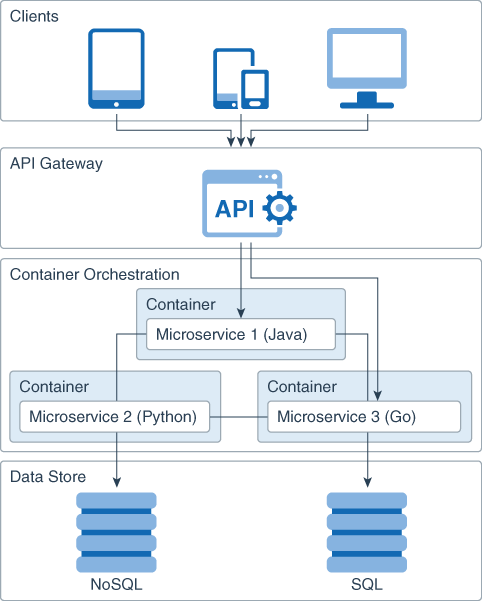
\includegraphics[scale=0.5]{Imagens/microservice_architecture.png}
	\end{center}
	\legend{Fonte: \citeonline{oracle_microservices}}
\end{figure}

Aplicações com uma arquitetura de microsserviços são separadas em partes, chamadas de microsserviços, que são classificadas e se comunicam por meio de uma rede. Microsserviços oferecem capacidades de negócio (funcionalidades relacionadas às regras de negócio da aplicação) ou capacidades de plataforma (funcionalidades relacionadas ao ambiente de execução da aplicação), tratando um aspecto em particular da aplicação. Eles se comunicam por meio de APIs bem definidas, contratos de dados, e configurações. O "micro" em microsserviços faz referência não ao tamanho do serviço, mas sim ao seu escopo de funcionalidade. Eles oferecem apenas uma determinada funcionalidade, tornando-se especialistas nela. Assim sendo, microsserviços não necessariamente devem ser pequenos em tamanho, mas fazem apenas uma tarefa e a fazem eficientemente. 
 
Sendo especialistas em apenas uma tarefa, microsserviços têm características e comportamentos que os diferenciam de outras arquiteturas orientadas a serviços, os quais serão discutidos no \autoref{chapter-caracteristicas}.

A \autoref{figura_arquitetura_microsservicos} exemplifica uma aplicação com arquitetura de microserviços. Inicialmente os usuários da aplicação (camada \emph{Clients}) fazem requisições à api para obter as informações desejadas. O \emph{API Gateway} - que é reponsável por integrar os serviços e será melhor discutido no \autoref{chapter-boas-praticas} - fará as devidas requisições para os devidos microsserviços (localizados na camada \emph{Container Orchestration}). Esses microsserviços então buscarão a informação necessária no devido banco de dados (camada \emph{Data Store}).

% A ilustração mostra as camadas da arquitetura de microsserviços. A primeira camada é a camada do cliente, que contém: os computadores, laptops e dispositivos móveis. A segunda camada é a camada do gateway de API, que redireciona as solicitações do cliente para os microsserviços apropriados. A terceira camada é a camada de orquestração de contêineres, com todos os microsserviços agrupados dentro de uma orquestração de contêineres. Cada um dos microsserviços está em contêiner. Eles se comunicam com os clientes por meio do gateway de API. A quarta camada é a camada de armazenamento de dados. Cada um dos microsserviços em contêiner que implementam persistência se comunica a apenas um armazenamento de dados. Os armazenamentos de dados exibidos são NoSQL e SQL.


% Microsserviços são uma abordagem arquitetônica e organizacional do desenvolvimento de software na qual o software consiste em pequenos serviços independentes que se comunicam usando APIs bem definidas. Esses serviços pertecem a pequenas equipes autossuficientes.

% A arquitetura de microsserviços (AMS) está ganhando força no desenvolvimento e entrega de aplicações de software como um conjunto de pequenos serviços granulares que podem ser integrados por meio de mecanismos de comunicação leve, normalmente APIs RESTful [10]. Microsserviços são componentes pequenos e facilmente entendíveis que possuem capacidades de negócio no meio dos serviços [11]. Esses serviços podem ser escalados independentemente (já que são desacoplados) pela implementação de \texttt{stacks} de tecnologias diferentes [2]. Muitos pesquisadores e praticantes dizem que AMS é uma evolução da Arquitetura orientada a serviços (AOS), como visto no contexto de serviços independentes/auto-suficientes e de natureza leve [12]. Por outro lado, AMS pode ser diferenciada da AOS em termos de compartilhamento de componentes, comunicação de serviços, mediação de serviços, e acesso remoto aos serviços [13]. (Bar, f., 2018, tradução nossa). \cite{WASEEM2020110798}
% % AOS é construida com base na ideia de compartilhar o máximo possível, enquanto AMS, o mínimo possível [13, 14]. AMS usa um estilo coreografico para comunicação inter-serviços, enquanto AOS aplica um estilo de orquestração para coordenação de serviços. Para mediação de serviços, AMS usa a camada de API que atua como uma fachada para o serviço, enquanto AOS adota o conceito de um \texttt{middleware} mensageiro para coodenação de serviços. Além disso, AMS em grande parte depende do protocolo REST e mensageria simples como protocolo de acesso remoto ao serviço; entretanto, AOS consegue lidar com diferentes tipos de protocolo de acesso remoto, incluindo mensageria simples para acessar serviços remotos [13].

\section{Trabalhos relacionados}

\subsection{{Microservices, IoT and Azure, por Bob Familiar - capítulo 2: What is a microservice}}

O capítulo 2 do livro de Bob Familiar descreve o que é um microsserviço, suas características e implicações, benefícios, e desafios. 

"Microservices do one thing and they do it well". Como é explicado por \citeonline{Familiar2015} , microsserviços representam business capabilities definidos usando o design orientado a domínio, são testados a cada passo do \emph{pipeline} de implantação, e lançados por meio de automação, como serviços independentes, isolados, altamente escaláveis e resilientes em uma infraestrutura em núvem distribuída. Pertecem a um time único de desenvolvedores, que trata o desenvolvimento do microsserviço como um produto, entregando software de alta qualidade em um processo rápido e iterativo com envolvimento do cliente e satisfação como métrica de sucesso.

\subsection{A Systematic Mapping Study on Microservices Architecture in DevOps, por Waseem, M., Liang, P. e Shahin, M.}

Esse trabalho tem o objetivo de sistematicamente identificar, analisar, e classificar a literatura sobre microsserviços em DevOps.

Inicialmente o leitor é contextualizado no mundo dos microsserviços e a cultura DevOps. Os autores usam a metodologia de pesquisa de um estudo de mapeamento sistemático da literatura publicada entre Janeiro de 2009 e Julho de 2018. Após selecionados 47 estudos, é feita a classificação deles de acordo com os critérios definidos pelos autores, e então é feita a discussão sobre os resultados obtidos - são expostos a quantidade de estudos sobre determinados tópicos em microsserviços, problemas e soluções, desafios, métodos de descrição, design patterns, benefícios, suporte a ferramentas, domínios, e implicações para pesquisadores e praticantes.

Os principais resultados são: (1) São identificados Três temas de pesquisa em AMS com DevOps “desenvolvimento e operações de microsserviços em DevOps”, “abordagens e suporte a ferramentas para sistemas baseados em AMS em DevOps”, e “Experiência de migração de AMS em DevOps”. (2) São identificados 24 problemas e apontadas suas respectivas soluções com respeito a implementação de microsserviços com DevOps. (3) A AMS é descrita princiapalmente usando caixas e linhas. (4) A maioria das qualidades da AMS são afetadas positivamente quando aplicadas com DevOps. (5) 50 ferramentas que suportam a construção de sistemas baseados em AMS são apontados. (6) A combinação da AMS e DevOps tem sido aplicada em uma ampla variedade de domínios de aplicações.


(Comparar cada trabalho com o meu trabalho. Coisas que eles não abordam e que eu abordo)

\chapter{Características}\label{chapter-caracteristicas}

\chapterprecis{Este capítulo aprensenta as propriedades e as vantagens dos microsserviços, assim como os desafios que acompanham suas implementações.}\index{sinopse de capítulo}

\section{Propriedades dos microsserviços}

\subsection{Autonomia e Isolamento}
Autonomia e isolamento significa que microsserviços são unidades auto-contidas de funcionalidade com dependências de outros serviços fracamente acopladas e são projetados, desenvolvidos, testados e lançados independentemente. O termo autônomo pode ser definido como - existe ou é capaz de existir independetemente das outras partes. O termo isolado, como - separado das outras partes. \cite{Familiar2015}

\subsection{Elasticidade, resiliência, e responsividade}

Microsserviços são reusados entre muitas soluções diferentes e portanto devem ser escaláveis de acordo com o uso. Devem ser resilientes, isso é, ser tolerantes a falhas e ter um tempo de recuperação razoável quando algo der errado. Além disso, devem ser responsivos, tendo um desempenho razoável de acordo com o uso. O termo elástico pode ser definido como - capaz de retornar ao tamanho/formato original depois de ser esticado, comprimido ou expandido. O termo resiliente, como - resistente às mudanças negativas. O termo responsivo, como - Rápido em responder e reagir. \cite{Familiar2015}

\subsection{Orientação-a-mensagens e programabilidade}

Microsserviços dependem de APIs e contratos de dados para definir como interagir com o serviço. A API define um conjunto de endpoints acessíveis por rede, e o contrato de dados define a estrutura da mensagem que é enviada ou retornada. O termo orientado-a-mensagens pode ser definido como - Software que conecta sistemas separados em uma rede, carregando e distribuindo mensagens entre eles. O termo programável, como - Obedece a um plano de tarefas que são executadas para alcançar um objetivo específico. \cite{Familiar2015}

\subsection{Configurabilidade}

Microsserviços devem provêr mais do que apenas uma API e um contrato de dados. Para que seja reusável e para que possa resolver as necessidades do sistema que o use, cada microsserviço tem níveis diferentes de configuração, e esta configuração pode ser feita de diferentes formas. O termo configurável pode ser definido como - Projetado ou adaptado para formar uma configuração ou para algum propósito. \cite{Familiar2015}

\subsection {Automação}

O ciclo de vida de um microsserviço deve ser totalmente automatizado, desde o planejamento (projeto) até a implantação. O termo automatizado pode ser definido como - Funcionar sem precisar ser controlado diretamente. \cite{Familiar2015}

\section{Vantagens}

\subsection{Evolução}

Quanto maior e mais antigo o software, mais difícil é de dar manutenção, e monólitos envelhecem com maior velocidade do que microsserviços. Entretanto, é possível migrar de um sistema monolítico para a arquitetura de microsserviços aos poucos, um serviço por vez, identificando capacidades de negócio, implementando-as como um microsserviço, e integrando com uso de padrões de baixo acoplamento. Ao longo do tempo, mais e mais funcionalidades podem ser separadas e implementadas como microsserviço, até que o núcleo da aplicação monolítica se transforme em apenas um outro serviço, ou um microsserviço. \cite{Familiar2015}

\subsection{Possibilidade de uso de diferentes ferramentas}

Cada microsserviço disponibiliza suas funcionalidades por meio de APIs e contratos de dados em uma rede. A comunicação independe da arquitetura que o microsserviço faz uso, então cada microsserviço pode escolher seu sistema operacional, linguagem e banco de dados. Isso é especialmente valioso para times com dificuldade de comunicação, pois cada time precisa apenas de conhecimento da arquitetura do microsserviço em que trabalha. \cite{Familiar2015}

\subsection{Alta velocidade}

Com um time responsável por cuidar do ciclo de desenvolvimento e sua automação, a velocidade com que microsserviços podem ser desenvolvidos é muito maior do que fazer o equivalente para uma solução monolítica. \cite{Familiar2015}

\subsection{Reusável e combinável}

Microsserviços são reusáveis por natureza. Eles são entidades independentes que provêm funcionalidades em um determinado escopo por meio de padrões de internet aberta. Para criar soluções para o usuário final, multiplos microsserviços podem ser combinados. \cite{Familiar2015}

\subsection{Flexibilidade no ambiente de execução}

A implantação de microsserviços é altamente dependente de sua automação. Para garantir flexibilidade de ambiente de execução, essa automação pode incluir configuração de cenários diferentes de uso, não apenas para produção, mas também para desenvolvimento e testagem, possibilitando que o microsserviço tenha o melhor desempenho em diversos cenários. Para tanto, é necessário o uso de ferramentas que configurem essa flexibilidade. \cite{Familiar2015}. Tais ferramentas serão melhor discutidas no \autoref{chapter-ferramentas}.

\subsection{Flexibilidade na escolha de tecnologias}

Cada microsserviço pode ser desenvolvido usando uma linguagem de programação e estrutura que melhor se adapte ao problema que ele é projetado para resolver, o que oferece mais possibilidades de tecnologias para usar. \cite{oracle_microservices}

\subsection{Versionável e substituível}

Com o controle completo dos cenários de implantação, é possível manter versões diferentes de um mesmo serviço rodando ao mesmo tempo, proporcionando retrocompatibilidade e fácil migração. Além disso, serviços podem ser atualizados ou mesmo substituidos sem ocasionar indisponibilidade do serviço. \cite{Familiar2015}


\section{Desafios}

De acordo com \citeonline{CAOPLE}, os três grandes desafios do desenvolvimento de aplicações com arquitetura de microsserviços são

1 - Como programar sistemas que consistem de um grande número de serviços executando em paralelo e distribuidos em um conjunto de máquinas;
% how to program systems that consists of a large number of services running in parallel and distributed over a cluster of computers;

2 - Como reduzir a sobrecarga de comunicação causada pela execução de grandes números de pequenos serviços;
%how to reduce the communication overhead caused by executing a large number of small services;

3 - Como sustentar a implantação flexível de serviços em uma rede para conseguir realizar o balanceamento de carga.
%how to support the flexible deployment of services to a network to achieve system load balance.

Esses e outros desafios podem ser dividos em tópicos mais específicos, abordados a seguir.

\subsection{Complexidade}
O uso da arquitetura de microsserviços implica num grande aumento de complexidade não apenas na infraestrutura, mas também em algumas etapas do ciclo de desenvolvimento do software, como no \emph{debug} ou nos testes por exemplo. Consequentemente, muitos outros desafios surgem a partir dessa complexidade. Além disso, o uso de diversas tecnologias pode trazer problemas por inexperiência dos desenvolvedores. De acordo com \citeonline{design-monitoring-testing-waseem}, mais pesquisas são necessárias para lidar com a complexidade dos microsserviços no nível de \emph{design} (projeto), de monitoramento, e de testes, desafios para qual não há soluções dedicadas.

% citar curso alura


% Desvantagens dos microserviços:
% - Maior complexidade de desenvolvimento e infraestrutura;
% - Debug mais complexo;
% - Comunicação entre os serviços deve ser bem pensada;
% - Diversas tecnologias pode trazer problemas por inexperiência dos devs;
% - Monitoramento é crucial e mais complexo;
% - (Criar um microserviço pode ser complexo, e ter demais pode trazer problemas.).

\subsection{Comunicação}

- Comunicação entre os serviços deve ser bem pensada

cross-platform compatibility issues and inconsistent call standards issues in the process of development and call microservices. \cite{ZUO2020102878}

\subsection{[re]Organizaçao}

Organizar o sistema e o time para sustentar uma arquitetura de microsserviços é um grande desafio. Como explica \citeonline{Familiar2015}: 
\begin{citacao}
    If you are part of a command-and-control organization using a waterfall software project management approach, you will struggle because you are not oriented to high-velocity product development. If you lack a DevOps culture and there is no collaboration between development and operations to automate the deployment pipeline, you will struggle. \cite{Familiar2015}
\end{citacao}

\subsection{Plataforma}
Criar o ambiente de execução para microsserviços requer um grande investimento em infraestrutura dinâmica em \emph{data centers} dispersos para garantir maior disponibilidade. Se sua atual plataforma \emph{on-premises} não suporta automação, infraestrutura dinâmica, escalamento elástico e alta disponibilidade, deve-se considerar uma plataforma na núvem. \cite{Familiar2015}. Mais sobre soluções na núvem será discutido no \autoref{chapter-ferramentas}.

\subsection{Identificação com DDD}

Domain-driven design (projeto orientado a domínio) é uma técnica bem consolidada e muito usada no desenvolvimento de software. Entretanto, para aplica-la em microsserviços, é necessário analisar onde cada peça desse padrão de projeto deve ficar. Veja a \autoref{praticas-identificacao-com-ddd} para um possível caminho a ser seguido.

% esse parágrafo não encaixa nas caracteristicas - desafios ?...

\subsection{Testes}

Assim como em qualquer aplicação, o teste é uma parte crucial do seu desenvolvimento. Escrever e testar código não muda muito entre as arquiteturas monolítica e de microsserviços, contudo, nos microserviços existem mais testes a serem executados. Não deve-se testar o microsserviço apenas antes de seu lançamento, mas sim em cada passo do \emph{pipeline} de implantação, sempre automatizando o máximo de etapas possível, para assim garantir uma entrega rápida de software de qualidade. \cite{Familiar2015}

% \subsection{Monitoramento}

\subsection{Descoberta}

Encontrar microsserviços em um ambiente distribuido pode ser feito de algumas maneiras diferentes. A informação pode ser armazenada diretamente no código, pode ser guardada e acessada em um arquivo, ou pode ser construido um microsserviço para encontrar outros microsserviços e disponibilizar suas localizações. Contudo, para prover detectabilidade como um serviço será necessário adquirir um produto de terceiros, integrar um projeto aberto, ou desenvolver sua própria solução. \cite{Familiar2015}

\chapter{Padrões}\label{chapter-padroes}

\section{Antes de tudo, o monólito}

\begin{citacao}
But as with any architectural decision there are trade-offs. In particular with microservices there are serious consequences for operations, who now have to handle an ecosystem of small services rather than a single, well-defined monolith. Consequently if you don't have certain baseline competencies, you shouldn't consider using the microservice style. \cite{MartinFowlerMicroservices}
\end{citacao}

\citeonline{MartinFowlerMicroservices} afirma que existem 3 pré-requisitos para se adotar uma arquitetura de microserviços, e que na grande maioria dos casos, deve-se começar pela arquitetura monolítica até que o sistema já esteja bem definido. Os pré-requisitos são - provisionamento rápido, monitoramento básico e deploy rápido de aplicação.

\subsection{Provisionamento rápido}

No contexto da computação, provisionamento significa disponibilizar um recurso, como uma máquina virtual por exemplo. Para produzir software, é necessário provisionar muitos recursos, tanto para os desenvolvedores quanto para o cliente. Naturalmente, o provisionamento é mais fácil na núvem. Na AWS por exemplo, para conseguir uma nova máquina, basta lançar uma nova instância e acessá-la - um processo muito rápido quando comparado ao \emph{on-premises}, onde precisaria-se comprar uma nova máquina, esperar chegar, configurá-la, e só então ela estará pronta. Para alcançar um provisionamento rápido, será necessário bastante automação.

\subsection{Monitoramento básico}

Muitas coisas podem dar errado em qualquer tipo de arquitetura, mas em especial nos microserviços pois cada serviço é fracamente acoplado, estando sujeitos não só a falhas no código, mas também na comunicação, na conexão, ou até falhas físicas. Portanto o monitoramento é crucial nesse tipo de arquitetura para que problemas, especialmente os mais graves possam ser detectados no menor tempo possível. Além disso, o monitoramento também pode ser usado para detectar problemas de negócio, como uma redução nos pedidos por exemplo.

\subsection{Deploy rápido de aplicação}

Na arquitetura de microserviços o deploy geralmente é feito separadamente para cada microserviço. Com muitos serviços para gerenciar, o deploy pode se tornar uma tarefa árdua, portanto será novamente necessário uma automação dessa etapa, que geralmente envolve um pipeline de deploy, que deve ser automatizado o máximo possível.

\section{Configuração}

\section{Deploy}

\section{Comunicação entre microserviços}

\section{Testes}

Mas além dos métodos mais conhecidos de testes, como test-driven development, teste de unidade e teste funcional, é necessário testar os microsserviços conforme passam pelo \emph{pipeline} de \emph{deploy}.

- Testes internos: Testar as funções internas do serviço, inclusive uso de acesso de dados, e caching.

- Teste de serviço: Testar a a implementação de serviço da API. Essa é uma implementação privada da API e seus modelos associados.

- Teste de protocolo: Testar o serviço no nível de protocolo, chamando a API sobre o determinado protocolo (geralmente HTTP).

- Composition Testing: Test the service in collaboration with other services within the context of a solution.

- Scalability/Throughput Testing: Test the scalability and elasticity of the deployed microservice.

- Failover/Fault Tolerance Testing: Test the ability of the microservice to recover after a failure.

- PEN Testing: Work with a third-party software security firm to perform penetration testing. NOTE: This will requires cooperation with Microsoft if you are pen testing microservices deployed to Azure.


\section{Como migrar do monolito para os microserviços}

\subsection{Identificação}

If you are currently working with a complex layered architecture and have a reasonable domain model defined, the domain model will provide a roadmap to an evolutionary approach to migrating to a microservice architecture. If a domain model does not exist, you can apply domain-driven design in reverse to identify the bounded contexts, the capabilities within the system. \cite{Familiar2015}

\subsection{Organização}

Em uma mudança do monolito para microsserviços, é recomendado que não sejam feitas mudanças grandes e abruptas na sua organização. Em vez disso, deve-se procurar uma oportunidade com uma iniciativa de negócio para testar a fórmula proposta por \citeonline{Familiar2015} : 

- Formar um pequeno time inderdisciplinar (cross-functional?).

- Oferecer treinamento e orientação na adoção de práticas ágeis, como o scrum.

- Oferecer uma localização física separada para esse time trabalhar a fim de não afetá-lo negativamente por politicas internas ou hábitos antigos.

- Adotar uma abordagem de minimo produto viável para entregar pequenos mas incrementais \emph{releases} de software, usando essa abordagem durante todo o ciclo de vida.

- Integrar esse serviço com sistemas existentes, usando um acoplamento solto.

- Percorrer esse ciclo de vida do microsserviço diversas vezes, fazendo as adaptações necessárias até chegar a equipe ficar confortável com o processo.

- Colocar o time principal em posições de liderança enquanto são formados novos times interdisciplinares para disseminar o conhecimento e a prática.
\chapter{Ferramentas}\label{chapter-ferramentas}
%https://dzone.com/articles/30top-tools-for-building-microservices-on-all-leve
\chapterprecis{Este capítulo aprensenta ferramentas que podem ser usadas na construção de aplicações com arquitetura de microsserviços}\index{sinopse de capítulo}

% \section{Design, testes, e monitoramento}

% De acordo com \citeonline{design-monitoring-testing-waseem}, mais pesquisas são necessárias para lidar com a complexidade dos microsserviços no nível de \emph{design} (projeto), de monitoramento, e de testes, desafios para qual não há soluções dedicadas.

Ferramentas de código aberto estão seguidas de um asterisco (*).

\section{Linguagens de programação}
Java, JavaScript, Python, Elixir

\section{Bancos de dados}

\subsection{Relacionais}
MySQL*, PostgreSQL*, MariaDB*

\subsection{Not-only SQL}
MongoDB*, Couchbase*, Redis*, Amazon DynamoDB

\section{Comunicação}

\subsection{RPC}
gRPC (\url{https://grpc.io/})

\subsection{Mensagens}
RabbitMQ*, Azure Service Bus, Amazon Simple Queue Service, Google Cloud Pub/Sub.

\subsection{Streaming de dados}
Apache Kafka*

\subsection{APIs}

\subsubsection{API Gateway}
Tyk*, Amazon API Gateway

\subsubsection{Linguagem de consulta}
GraphQL*

\subsubsection{Documentação}
Swagger Inspector

% \subsection*{GraphQL}
% A query language for your API
% GraphQL is a query language for APIs and a runtime for fulfilling those queries with your existing data. GraphQL provides a complete and understandable description of the data in your API, gives clients the power to ask for exactly what they need and nothing more, makes it easier to evolve APIs over time, and enables powerful developer tools. \cite{GraphQL-site}

\subsubsection{Testes de API}\label{ferramentas-testes-apis}
Postman*, Hoppscotch*, API Fortress

% RapidAPI offers RapidAPI Client for VS Code to test APIs locally inside Visual Studio Code. You can also schedule API tests using RapidAPI Studio.
% programar os testes em uma linguagem de programação
% cURL
% postman
% solução integrada ao VSCode - thunderclient

\section{Provisionamento}

\subsection*{de máquinas virtuais}
VirtualBox*

\subsection*{de containers}
Docker*

\subsection*{na núvem}
AWS EC2

\subsection*{automático}
AWS Launch Templates

\section{Escalamento}
AWS Auto Scaling Groups

% \subsection{Ferramentas para segurança em APIs}

% Autenticação - Always use secure authentication methods such as OAuth, JWTs, or API Keys. It's not recommended to use basic HTTP authentication as it sends user credentials with each request. It is considered the least secure method.

% Validação de entradas - Métodos de validação de entrada: JSON and XML Schema validation; Regular expressions;  Data type validators available in framework; Minimum and maximum value range check for numerical inputs;  Minimum and maximum length check for strings.

% \subsubsection{Métodos de autenticação}

% API Keys are unique identifiers assigned to clients, which grant them access to an API. They are passed to the server with every request and authenticate the client. They also provide authorization and can be used to identify a user's individual access permissions. API Keys are long alphanumerical strings designed to be almost impossible to guess. They are passed to servers as a query parameter or in an HTTP request header.

% OAuth is a powerful framework that uses tokens to give apps limited access to a user’s data without needing the user’s password. The tokens used are restricted and only allow access to data that the user specified for the particular app. It works by the user(client) first requesting authorization from the resource owner. The user is then given a unique access token from an authorization server used in each request to the resource server.

% Basic HTTP authentication involves the client passing the user’s username and password with every request. This is done using an HTTP Header. Basic HTTP authentication is generally considered the least secure. However, if you decide to use it, ensure you are using an HTTPS connection. If not, data is a risk of being leaked.

% Ferramenta para rate limiting. \cite{rapidAPI-twitter}

\section{Orquestração}

Docker Swarm*, Kubernetes*, Conductor*, Azure Kubernetes Service (AKS)

% Learn About Orchestrating Microservices Using Kubernetes

% The microservices that are running in containers must be able to interact and integrate to provide the required application functionalities. This integration can be achieved through container orchestration.

% Container orchestration enables you to start, stop, and group containers in clusters. It also enables high availability and scaling. Kubernetes is one of the container orchestration platforms that you can use to manage containers.

% After you containerize your microservices, you can deploy them to Oracle Cloud Infrastructure Container Engine for Kubernetes.

% Before you deploy your containerized microservices application to the cloud, you must deploy and test it in a local Kubernetes engine, as follows:

%     Create your microservices application.
%     Build Docker images, to containerize your microservices.
%     Run your microservices in your local Docker engine.
%     Push your container images to a container registry.
%     Deploy and run your microservices in a local Kubernetes engine, such as Minikube.

% After testing the application in a local Kubernetes engine, deploy it to Oracle Cloud Infrastructure Container Engine for Kubernetes as follows:

%     Create a cluster.
%     Download the kubeconfig file.
%     Install kubectl tool on a local device.
%     Prepare the deployment.yaml file.
%     Deploy the microservice to the cluster.
%     Test the microservice.

% The following diagram shows the process for deploying a containerized microservices application to Oracle Cloud Infrastructure Container Engine for Kubernetes. 

\section{Monitoramento}
Logstash*, Middleware, Elastic Stack, Graylog*

\section{Conjunto de ferramentas}
Seneca*, Google Cloud Functions,

\section{Framework arquitetural}
goa*, Kong*

\section{Ferramentas sem servidor}
Claudia, Apache Openwhisk, Serverless, Kubeless, IronFunctions, AWS Lambda, OpenFaaS, Microsoft Azure Functions.

% \section{Plataformas}
% Microsoft Azure is a microservice platform, and it provides a fully automated dynamic infrastructure, SDKs, and runtime containers along with a large portfolio of existing microservices that you can leverage, such as DocumentDb, Redis In-Memory Cache, and Service Bus, to build your own microservices catalog. \cite{Familiar2015}
% AWS
% Uma solução para a sobrecarga na execução de tantos microserviços é a um ambiente de desenvolvimento integrado na linguagem CAOPLE \cite{CAOPLE}. Essa plataforma oferece grande controle sobre a implantação e testagem de microserviços.
\chapter{Conclusão}\label{chapter-conclusao}

As conclusões constituem a parte final do texto, na qual se apresentam as considerações finais sobre o assunto, se os objetivos foram alcançados, o que se descobriu, quais outras questões surgiram a partir dos resultados e se as hipóteses se confirmaram ou não. Vale lembrar que nenhum trabalho de pesquisa encerra um tema ou problema, por isso, evite fazer afirmações redutoras ou definitivas.
\chapter*{Plano de Continuidade}

Analisar a eficiência desses padrões e práticas.

Analisar a eficiência dessas soluções e ferramentas.

Explicar e detalhar as ferramentas.

Propor uma combinação desses padrões e dessas ferramentas para a construção de uma aplicação exemplar com arquitetura de microsserviços.


Diagrama de gantt \url{https://www.seomartin.com/modelo-diagrama-de-gantt/}

Atividade | tabela

\phantompart
\bibliography{Bibliografia}

%%%%%%%%%%%%%%%%%%%%%%%%%%%%%%%%%%%%%%%%%%%%%%%%%%%%%%%%%%%%%%%%%%%%%%%%%%
% ELEMENTOS PÓS-TEXTUAIS
%%%%%%%%%%%%%%%%%%%%%%%%%%%%%%%%%%%%%%%%%%%%%%%%%%%%%%%%%%%%%%%%%%%%%%%%%%

\postextual

\renewcommand{\chapnumfont}{\chaptitlefont}
\renewcommand{\afterchapternum}{}
\include{Pos_Textual/Apendices}
\include{Pos_Textual/Anexos}

\end{document}
